\documentclass[10pt,a4paper,twocolumn]{article}
% ------------------------------------------------------------------ packages
\usepackage[T1]{fontenc}
\usepackage[utf8]{inputenc}
\usepackage{lmodern}
\usepackage[a4paper,left=21.5mm,right=21.5mm,top=24mm,bottom=24mm,columnsep=7mm,headsep=8mm]{geometry}
\usepackage{amsmath,amssymb}
\usepackage{graphicx}
\usepackage{xcolor}
\usepackage{booktabs,tabularx,multirow,array}
\usepackage{adjustbox}
\usepackage{stfloats}
\usepackage{enumitem}
\usepackage{titlesec}
\usepackage{fancyhdr}
\usepackage[labelfont=bf,font=small,labelsep=colon,skip=4pt]{caption}
\usepackage{subcaption}
\usepackage{tikz}
\usetikzlibrary{arrows.meta,positioning,backgrounds}
\usepackage[hidelinks]{hyperref}
\usepackage{microtype}

% ------------------------------------------------------------------ styling
\definecolor{navy}{RGB}{31,56,100}
\definecolor{dsred}{RGB}{200,30,30}
\definecolor{fGreen}{RGB}{220,250,220}  \definecolor{dGreen}{RGB}{20,130,20}
\definecolor{fOrange}{RGB}{253,238,222} \definecolor{dOrange}{RGB}{190,95,0}
\definecolor{fRed}{RGB}{253,225,230}    \definecolor{dRed}{RGB}{180,20,30}
\definecolor{fBlue}{RGB}{228,228,252}   \definecolor{dBlue}{RGB}{30,30,150}
\definecolor{fYellow}{RGB}{255,250,190} \definecolor{fGray}{RGB}{240,240,240}

\newcommand{\nm}[1]{{\color{dsred}\textbf{#1}}}   % not (yet) measured
\newcommand{\code}[1]{\texttt{#1}}

\titleformat{\section}{\Large\bfseries\color{navy}}{\thesection.}{0.5em}{}
\titleformat{\subsection}{\large\bfseries}{\thesubsection}{0.6em}{}
\titlespacing*{\section}{0pt}{9pt plus 2pt}{5pt}
\titlespacing*{\subsection}{0pt}{7pt plus 2pt}{3pt}

\pagestyle{fancy}
\fancyhf{}
\fancyhead[C]{\small\itshape DriveShieldX: Smart Traffic Violation and Road Safety Monitoring System}
\fancyfoot[C]{\thepage}
\renewcommand{\headrulewidth}{0.4pt}
\fancypagestyle{plain}{\fancyhf{}\fancyhead[C]{\small\itshape DriveShieldX: Smart Traffic Violation and Road Safety Monitoring System}\fancyfoot[C]{\thepage}\renewcommand{\headrulewidth}{0.4pt}}

\setlist[itemize]{leftmargin=1.1em,itemsep=1pt,topsep=2pt,parsep=0pt}
\setlist[enumerate]{leftmargin=1.5em,itemsep=1pt,topsep=2pt,parsep=0pt}
\setlength{\parskip}{0pt}
\renewcommand{\arraystretch}{1.08}

\hypersetup{pdftitle={DriveShieldX: Smart Traffic Violation and Road Safety Monitoring System},
            pdfauthor={Heli Makwana, Nisha Mandal, Tanisha Sankhe, Sonal Kadam}}

\begin{document}
% ================================================================== TITLE
\twocolumn[{%
\begin{center}
{\LARGE\bfseries DriveShieldX: Smart Traffic Violation and Road Safety\\[2pt]
Monitoring System Using YOLOv8, Centroid-Based\\[2pt]
Tracking, and Multi-Violation Detection\par}
\vspace{8pt}
{\large\bfseries Heli Makwana\textsuperscript{1}, Nisha Mandal\textsuperscript{2}, Tanisha Sankhe\textsuperscript{3}, and Sonal Kadam\textsuperscript{4}\par}
\vspace{5pt}
{\small
\textsuperscript{1}Student, Department of Computer Science and Technology, Usha Mittal Institute of Technology,\\ SNDT Women's University, Mumbai, India\\
\textsuperscript{2}Student, Department of Computer Science and Technology, Usha Mittal Institute of Technology,\\ SNDT Women's University, Mumbai, India\\
\textsuperscript{3}Student, Department of Computer Science and Technology, Usha Mittal Institute of Technology,\\ SNDT Women's University, Mumbai, India\\
\textsuperscript{4}Assistant Professor, Department of Computer Science and Technology, Usha Mittal Institute of Technology,\\ SNDT Women's University, Mumbai, India\\[3pt]
Email -- \textsuperscript{1}helimakwana969@gmail.com, \textsuperscript{2}nishamandal2855@gmail.com,\\
\textsuperscript{3}tanishasankhe07@gmail.com, \textsuperscript{4}sonalkadam0312@gmail.com\par}
\end{center}
\vspace{4pt}
\begin{list}{}{\leftmargin=6mm\rightmargin=6mm}\item\small\itshape
\textbf{Abstract:} Enforcement of traffic law in Indian cities is still carried out largely by eye: an officer sees one
junction, so a rider who passes one signal bare-headed and speeds a kilometre on is recorded, if at all, as two
unconnected events. DriveShieldX is built around that discontinuity. One pipeline consumes CCTV video and reasons about
four infringements at once --- no helmet, no seat belt, triple-riding and over-speeding --- with YOLOv8 [1] detecting,
ByteTrack [6] holding one identity per vehicle so that every flag accrues to one record, a two-stage ANPR stage
recovering the plate, and an e-challan composed automatically only when the evidence is unambiguous and the plate is
verified against a registry; a disagreement rule routes the clip to a reviewer when a dedicated helmet classifier and
the combined detector conflict. Every component is measured on independent ground truth. On ten UA-DETRAC sequences
ByteTrack reaches IDF1 75.2 with 3.5$\times$ fewer identity switches than centroid association and IDF1 equal to
DeepSORT at 357$\times$ its association speed. On 281 human-reviewed helmet events the gate cuts false issuance from
21.0\% to 1.1\%. On 291 held-out Indian plates localisation recall is 99.3\% and a plate-specific recogniser raises
exact reading from 16.5\% to 36.8\% at a tenth of the cost. A video model fine-tuned on 127 hand-labelled crashes
detects 7 of 23 held-out UCF-Crime crashes at 3.9 false alarms per hour, against 1 of 23 for trajectory rules, and the
fog index separates fog from clear footage with ROC AUC 0.95. The record then flows without a manual step into Motor
Vehicles Act penalties, repeat-offender licence action, SMS notice, self-settling online payment and an unpaid-challan
escalation path modelled on Indian procedure. Plate reading, CPU throughput (0.26--1.66 FPS) and speed calibration
remain the weakest points.
\end{list}
\vspace{2pt}
{\small\noindent\textbf{Keywords:} YOLOv8, traffic violation detection, ANPR, helmet detection, ByteTrack, multi-object
tracking, accident detection, e-challan, intelligent transportation systems\par}
\vspace{10pt}
}]

% ================================================================== 1
\section{Introduction}
\subsection{Traffic Violation and Road Safety Crisis}
Indian roads claim in excess of 1.5 lakh lives annually. The dominant causes are not exotic ---
unhelmeted riders, unbelted occupants and excessive speed account for the bulk of them --- and statutes covering all
three already exist [26]. What fails is enforcement.

A constable can occupy one position at a time, and observation by eye is slow, inconsistent and readily contested.
Cities have installed CCTV by the thousand, yet most streams are unattended or consulted only after a collision. What
is absent is a system that watches the feeds continuously and acts on what it sees.

\subsection{Limitations of Existing Systems}
Deployed monitoring installations tend to be single-purpose. A speed camera measures speed. A helmet rig inspects
heads. Neither exchanges information with the other. Should one motorcycle omit a helmet, breach the limit and carry
three occupants during a single trip, the outcome is three disconnected records --- or no record whatsoever. Five
recurring deficiencies motivated this work.
\begin{itemize}
\item \textbf{Violations are never correlated.} Three infringements by one vehicle ought to constitute one record
carrying three flags, not three unrelated entries.
\item \textbf{Databases are not live.} An officer downstream needs the violation within seconds, not the next morning.
\item \textbf{Challan generation stays manual.} Detection is automated, the paperwork is not, which reintroduces
precisely the bottleneck automation was meant to remove --- and when it is automated, a misread plate sends the notice
to the wrong citizen.
\item \textbf{Weather and incident monitoring are separate products.} Fog assessment and crash alerting run in their
own applications, despite fog being exactly the condition under which detection degrades and collisions become likelier.
\item \textbf{Model uncertainty is ignored.} If the network fires, the challan issues; no step defers a marginal
prediction to a person. An erroneous challan costs a citizen leave from work and a court appearance --- a heavy burden
to impose because a confidence score read 0.51 rather than 0.85.
\end{itemize}

\subsection{Proposed Solution and Contributions}
DriveShieldX consolidates what are ordinarily five separate systems into one. Its contributions are:
\begin{enumerate}
\item \textbf{A unified four-violation pipeline.} Helmet absence, seat-belt absence, triple-riding and over-speeding
are evaluated inside a single per-frame inference cycle rather than by independently executed detectors.
\item \textbf{Identity-preserving violation aggregation.} ByteTrack assigns one persistent identity per vehicle, so
every flag raised along a trajectory is written to a single enforcement record; we measure that identity persistence
against published ground truth.
\item \textbf{An explicit uncertainty gate.} A standalone helmet classifier and the combined multi-class detector are
executed side by side. Agreement issues the challan; disagreement forwards the event for human review. On
human-reviewed events this reduces wrong automatic challans by a factor of nineteen.
\item \textbf{Verified, end-to-end enforcement.} Detection feeds ANPR, ANPR feeds a registry check, and only a
verified plate leads to an automatic challan; notice, payment, repeat-offender licence action and escalation of unpaid
challans follow without a manual step.
\item \textbf{A road-safety layer on the same feed.} A learned crash detector and a fog index consume the same frames
and dispatch alerts to the nearest police station and hospital.
\item \textbf{An evaluation that states its own boundary.} The experimental setup documents data and provenance; the
results report what has been measured, on independent ground truth, and with equal prominence what has not.
\end{enumerate}

% ================================================================== 2
\section{Literature Review}
Published work divides into studies that perfect one task in isolation and integrated systems that attempt several
tasks at once, usually surrendering some precision in exchange.

\subsection{Single-Task Detection Systems}
Suman et al.\ [13] report 99.3\% mAP for helmet detection with YOLOv11, Sutikno et al.\ [14] 87--92\% on seat-belt
compliance using YOLOv8 with contrast limited adaptive histogram equalisation [19], and Gautam and Kumar [15] hold
monocular speed error to roughly $\pm$2--3 km/h by pairing centroid tracking with Kalman smoothing. Plate pipelines on
YOLOv8 with EasyOCR [20] generally settle between 90\% and 94\% [3]. Every number here is quoted from the cited
authors' publications; none is ours.

Such scores come from curated datasets of clear views, whereas operational CCTV carries occlusion, oblique geometry,
motion blur and low light; Section~5 therefore documents data before any figure is quoted.

\subsection{Multi-Task and Integrated Systems}
Among integrated designs, M.\,R.\ et al.\ [17] report 93--97\% on unified detection, Kejriwal et al.\ [16] 92.3\%
mAP@0.5 for counting with YOLOv8 and DeepSORT, and Lin and Jhang [12] 92.0\% at 37.9 FPS for flow monitoring by
combining YOLOv5 with convolutional fuzzy neural networks; Srinath et al.\ [4] couple vehicle recognition with
e-challan generation. Accident detection is usually posed standalone; Qamar et
al.\ [18] report 96.76\% using CNN-based motion analysis, while surveillance benchmarks such as UCF-Crime [23] show how
hard crashes are to detect in low-resolution, distant CCTV.

\subsection{Multi-Object Tracking}
Because a violation attaches to a vehicle rather than a frame, the tracker is as consequential as the detector.
SORT [7] matches detections across frames with a Kalman filter and Hungarian assignment on IoU alone; DeepSORT [5] adds
an appearance embedding, reducing identity switches through occlusion at the cost of a network evaluation per track
per frame; ByteTrack [6] instead retains low-confidence boxes as second-stage association candidates, attaining strong
MOTA and IDF1 on MOT17 with no appearance model. Centroid association --- nearest-neighbour matching on box centres
under a Euclidean gate --- is cheapest and widely used in traffic work [2], yet its behaviour in dense scenes is rarely
quantified against stronger trackers. Evaluation follows the established protocol: MOTA [8], IDF1 [9] and HOTA [10],
as defined for the MOT benchmarks [11].

\subsection{Research Gaps Addressed}
The deficiencies enumerated in the introduction recur throughout this literature: no work surveyed correlates several
infractions to one vehicle identity, none carries detection through ANPR and a registry check to challan issuance
without a manual step, weather and collision analysis are published as standalone systems although they consume the
identical feed, and no pipeline interposes a state in which a low-confidence prediction is deferred to a person rather
than acted upon. DriveShieldX addresses all four.

% ================================================================== 3
\section{Objectives}
We set out to build one pipeline that recognises four violation categories from ordinary CCTV using YOLOv8; to hold a
single identity per vehicle across frames --- by ByteTrack, with the centroid associator as the
lightweight fallback --- so that multiple infringements resolve to one record; to recover plate numbers through a
two-stage ANPR flow and verify them against a registry before an automated challan is composed; to interpose a
disagreement rule that suspends issuance when the standalone and combined models conflict; to add crash and fog
monitoring on the same feed; and to evaluate all of it on documented data with independent ground truth, decomposed by
ablation and reported with dispersion and significance where repeated observations exist --- and, where an
evaluation could not be completed, to say so explicitly rather than to substitute an unsupported figure.

% ================================================================== 4
\section{Research Methodology}
\begin{figure*}[t]
\centering
\resizebox{\textwidth}{!}{%
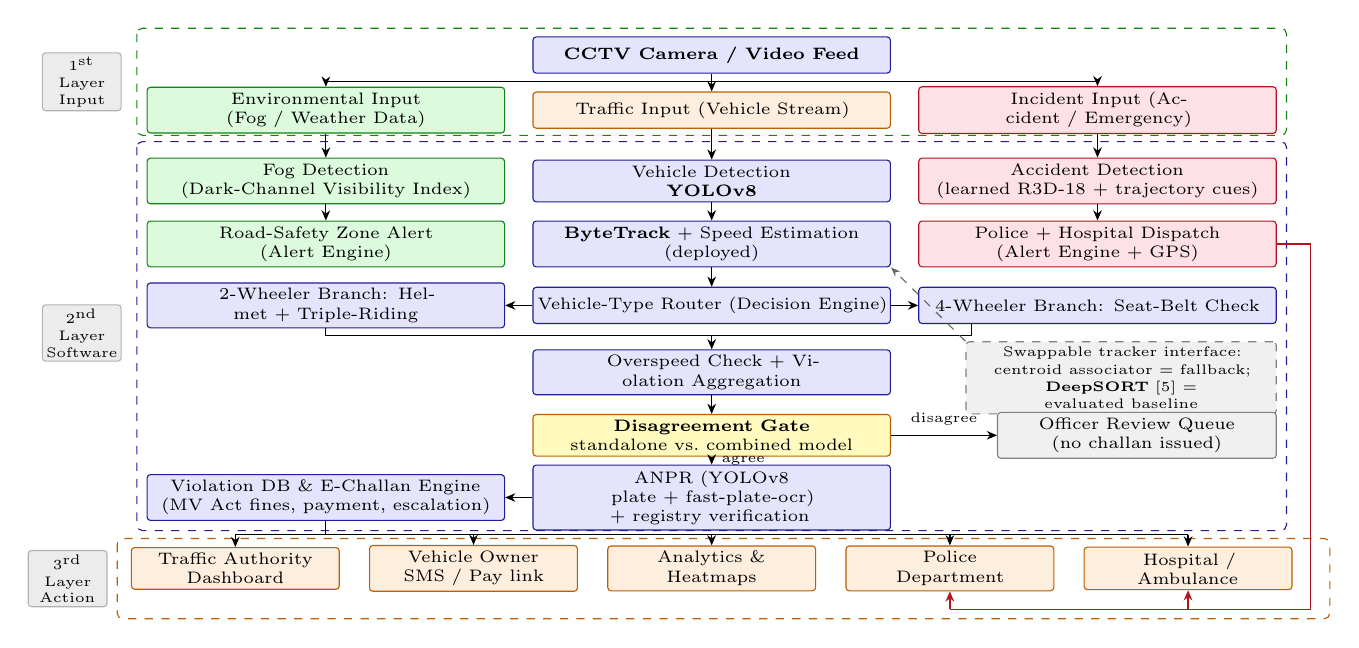
\begin{tikzpicture}[x=1mm,y=1mm,font=\fontsize{6}{6.9}\selectfont,
  bx/.style={draw,rounded corners=1.2pt,align=center,text width=44mm,minimum height=4.6mm,inner sep=0.7mm,line width=0.4pt},
  gB/.style={bx,draw=dGreen,fill=fGreen},
  oB/.style={bx,draw=dOrange,fill=fOrange},
  rB/.style={bx,draw=dRed,fill=fRed},
  bB/.style={bx,draw=dBlue,fill=fBlue},
  yB/.style={bx,draw=dOrange,fill=fYellow},
  aB/.style={bx,draw=dOrange,fill=fOrange,text width=25mm},
  tag/.style={draw=gray!60,fill=gray!15,rounded corners=1.2pt,align=center,text width=9mm,inner sep=0.5mm,font=\fontsize{5.2}{6}\selectfont},
  ar/.style={-{Stealth[length=1.3mm,width=1.1mm]},line width=0.45pt},
  ln/.style={line width=0.45pt},
  lb/.style={font=\fontsize{4.8}{5}\selectfont}]
\def\E{36}\def\T{85}\def\I{134}
\node[bB,font=\fontsize{6}{6.9}\selectfont\bfseries] (cctv) at (\T,0) {CCTV Camera / Video Feed};
\node[gB] (env) at (\E,-7) {Environmental Input (Fog / Weather Data)};
\node[oB] (tin) at (\T,-7) {Traffic Input (Vehicle Stream)};
\node[rB] (iin) at (\I,-7) {Incident Input (Accident / Emergency)};
\node[gB] (fog)  at (\E,-16) {Fog Detection\\(Dark-Channel Visibility Index)};
\node[bB] (vdet) at (\T,-16) {Vehicle Detection\\\textbf{YOLOv8}};
\node[rB] (acc)  at (\I,-16) {Accident Detection\\(learned R3D-18 + trajectory cues)};
\node[gB] (zone) at (\E,-24) {Road-Safety Zone Alert\\(Alert Engine)};
\node[bB] (trk)  at (\T,-24) {\textbf{ByteTrack} + Speed Estimation\\(deployed)};
\node[rB] (disp) at (\I,-24) {Police + Hospital Dispatch\\(Alert Engine + GPS)};
\node[bB] (tw)   at (\E,-31.8) {2-Wheeler Branch: Helmet + Triple-Riding};
\node[bB] (rtr)  at (\T,-31.8) {Vehicle-Type Router (Decision Engine)};
\node[bB] (fw)   at (\I,-31.8) {4-Wheeler Branch: Seat-Belt Check};
\node[bB] (agg)  at (\T,-40.3) {Overspeed Check + Violation Aggregation};
\node[bx,draw=gray,dashed,fill=fGray,text width=38mm,font=\fontsize{5.4}{6.2}\selectfont] (note) at (\I+3,-41.0) {Swappable tracker interface:\\centroid associator = fallback;\\\textbf{DeepSORT} [5] = evaluated baseline};
\node[yB] (gate) at (\T,-48.3) {\textbf{Disagreement Gate}\\standalone vs.\ combined model};
\node[bx,draw=gray,fill=fGray,text width=34mm] (rev) at (\I+5,-48.3) {Officer Review Queue\\(no challan issued)};
\node[bB] (anpr) at (\T,-56.2) {ANPR (YOLOv8 plate + fast-plate-ocr)\\+ registry verification};
\node[bB] (db)   at (\E,-56.2) {Violation DB \& E-Challan Engine\\(MV Act fines, payment, escalation)};
\node[aB] (a1) at (24.5,-65.2)  {Traffic Authority\\Dashboard};
\node[aB] (a2) at (54.75,-65.2) {Vehicle Owner\\SMS / Pay link};
\node[aB] (a3) at (85,-65.2)    {Analytics \&\\Heatmaps};
\node[aB] (a4) at (115.25,-65.2){Police\\Department};
\node[aB] (a5) at (145.5,-65.2) {Hospital /\\Ambulance};
\begin{scope}[on background layer]
 \draw[dGreen,dashed,rounded corners=2pt] (12,3.4) rectangle (158,-10.2);
 \draw[dBlue,dashed,rounded corners=2pt] (12,-11.0) rectangle (158,-60.4);
 \draw[dOrange,dashed,rounded corners=2pt] (9.5,-61.4) rectangle (163.5,-71.6);
\end{scope}
\node[tag] at (5,-3.4)  {1\textsuperscript{st} Layer\\Input};
\node[tag] at (5,-35.3) {2\textsuperscript{nd} Layer\\Software};
\node[tag] at (3.2,-66.5) {3\textsuperscript{rd} Layer\\Action};
\draw[ln] (cctv.south) -- (\T,-3.4);
\draw[ln] (\E,-3.4) -- (\I,-3.4);
\foreach \n/\x in {env/\E,tin/\T,iin/\I} \draw[ar] (\x,-3.4) -- (\n.north);
\draw[ar] (env) -- (fog);  \draw[ar] (tin) -- (vdet); \draw[ar] (iin) -- (acc);
\draw[ar] (fog) -- (zone); \draw[ar] (vdet) -- (trk); \draw[ar] (acc) -- (disp);
\draw[ar] (trk) -- (rtr);
\draw[ar] (rtr) -- (tw);   \draw[ar] (rtr) -- (fw);
\draw[ln] (tw.south) -- (\E,-35.6) -- (\I-16,-35.6) -- (\I-16,-34.1);
\draw[ar] (\T,-35.6) -- (agg.north);
\draw[ar] (agg) -- (gate);
\draw[ar] (gate) -- node[above,lb]{disagree} (rev);
\draw[ar] (gate) -- node[right,lb]{agree} (anpr);
\draw[ar] (anpr) -- (db);
\draw[-{Stealth[length=1.2mm]},dashed,gray!80!black,line width=0.4pt] (note.north west) -- (trk.south east);
\draw[ln] (db.south) -- (\E,-60.9);
\draw[ln] (24.5,-60.9) -- (145.5,-60.9);
\foreach \n/\x in {a1/24.5,a2/54.75,a3/85,a4/115.25,a5/145.5} \draw[ar] (\x,-60.9) -- (\n.north);
\draw[ln,dRed] (disp.east) -- (161,-24) -- (161,-70.4) -- (115.25,-70.4);
\draw[ar,dRed] (115.25,-70.4) -- (a4.south);
\draw[ar,dRed] (145.5,-70.4) -- (a5.south);
\end{tikzpicture}}
\caption{DriveShieldX system architecture. The deployed configuration tracks with ByteTrack; the centroid associator
is the fallback at the same interface and DeepSORT is implemented as an evaluated baseline (Section~6.3). The
disagreement gate is the single point at which an automatic challan can be suppressed in favour of human review, and
only a registry-verified plate leads to an automatic challan.}
\end{figure*}

\subsection{System Architecture and Data Flow}
The pipeline is modular (Figure~1). Raw frames enter pre-processing; YOLOv8 then detects on each frame. Every
detected vehicle receives an identifier and passes to the tracker, which maintains that identifier across frames and
supplies the displacement history used for speed estimation. Vehicle class --- two-wheeler or four-wheeler --- selects
the violation branch that executes next. All raised flags are collected before ANPR reads the plate, the plate is
verified against the vehicle registry, and the completed record is written to the Violation Database, from which the
e-Challan engine notifies the registered owner and the Traffic Authority. Fog assessment and accident detection
consume the same frames on separate threads and so do not extend the latency of the primary path.

\subsection{Object Detection Backbone}
YOLOv8 [1] is the primary detector: each frame passes through the network once, yielding boxes, class labels and
confidences. Five weight sets are loaded concurrently --- \code{person}, \code{twowheeler}, \code{helmet},
\code{seatbelt} and \code{plate} --- the four task models initialised from COCO pre-training and fine-tuned on the
corresponding dataset of Section~5.1. The single-pass design, multi-scale aggregation and tolerance of partial
occlusion recommend it for surveillance video, where distant riders and dense queues occur in the same frame.

\subsection{Tracking and Speed Estimation}
ByteTrack associates detections across frames and supplies the persistent identity on which violation aggregation
depends. The fallback centroid associator takes each box midpoint $(c_x,c_y)$ and matches centroids in consecutive
frames by minimum Euclidean distance subject to a gating radius $\tau_d$, retaining an unmatched track for $\tau_a$
frames before deletion so that short detection dropouts are absorbed. Either tracker supplies the displacement history
from which vehicle speed is estimated using centroid displacement, frame rate, and a pixel-to-real-world calibration
factor [15]:
\begin{equation}
\begin{aligned}
v &= \frac{d_{\mathrm{real}}\times \mathrm{FPS}}{N_{\mathrm{frames}}}\times 3.6 \quad (\mathrm{km/h}),\\
d_{\mathrm{real}} &= s_{px}\cdot \lVert \mathbf{c}_t-\mathbf{c}_{t-N}\rVert_2
\end{aligned}
\end{equation}
where $s_{px}$ is a pixel-to-metre scale and $N_{\mathrm{frames}}$ the frames elapsed between reference lines. Both
terms are sources of the error analysed in Section~6.4: $s_{px}$ is presently a single uncalibrated constant of 0.045
shared by every camera, and the frame rate substituted for FPS is fixed at 25.0 rather than read from the clip. Since
the first version of this work, a plausibility hold prevents any reading above 200 km/h from becoming a penalty: such
a reading is marked disputed and sent to an officer.

\subsection{Multi-Violation Detection Modules}
\textbf{Helmet (two-wheeler branch).} A YOLOv8 model trained on \code{helmet}/\code{no\_helmet} instances evaluates the
rider head region inside each detected motorcycle box; absence raises a \code{no\_helmet} event.
\textbf{Triple-riding (two-wheeler branch).} Person detections whose boxes intersect a two-wheeler box above an overlap
threshold are counted, and a count exceeding two logs a \code{three\_seater} event against that track.
\textbf{Seat belt (four-wheeler branch).} The occupant associated with a car is cropped and classified for belt
presence, with CLAHE [19] applied beforehand to recover contrast under low light and glare. Because occupants behind
glass are often missed by the person detector, a car with no associated person is now checked on its windscreen band
and on its driver and passenger halves instead of being skipped; a violation still requires the no-belt score to beat
the belt score by a margin.
\textbf{Over-speed.} The speed of Equation~(1) is compared against a per-camera, per-zone limit and graded into low,
medium, high and extreme bands.
\textbf{Aggregation and the disagreement gate.} All flags active for a track are merged before ANPR is invoked, so one
challan carries every concurrent infraction. Immediately before issuance the gate compares the standalone helmet
classifier against the combined multi-class detector on the same crop. With $p_s$ and $p_c$ their positive-class
confidences and $\theta$ the issuance threshold, a challan is composed automatically only if both exceed $\theta$ or
both fall below it; otherwise the event is written to the officer review queue with its evidence crop and no notice is
dispatched. Section~6.6 measures what the gate buys.

\subsection{ANPR, Registry Verification and Challan Generation}
ANPR operates in two stages. A YOLOv8 model localises the plate; the crop is padded on both sides, where the state
code sits, and read by a plate-specific recogniser, fast-plate-ocr [24], a small ONNX model trained on plate crops, with
EasyOCR [20] retained as a fallback when the recogniser is unavailable. Indian plate grammar --- a valid state code,
district number, series and four-digit number, or the Bharat series --- is then used to repair look-alike glyphs
(0/O, 1/I, 2/Z, 5/S, 8/B) by position.

Only a read that is a valid registration and is found in the vehicle registry leads to an automatic challan; a
missing, malformed or unregistered plate is not fined but placed before an officer with the reason recorded. The
registry is the system's own table of registered vehicles, behind a provider interface to which a Vahan/RC lookup can
be attached without code change. The e-Challan engine applies the statutory penalties of the Motor Vehicles
(Amendment) Act 2019 [26] --- Rs~1000 and a three-month disqualification for riding without a helmet (s.~194D), Rs~1000
and three months for triple-riding (s.~194C), Rs~1000 for not wearing a seat belt (s.~194B) --- or a graduated
schedule (Rs~500, 1000, 3000 within 365 days), whichever is higher. A third offence, or five challans in a year,
suspends the licence; the strike cycle restarts once a suspension ends, but no challan or suspension is ever deleted
from the driver's record. Notice goes by SMS with a payment link; payment is confirmed by a signed redirect, a signed
webhook and periodic reconciliation with the gateway, and settlement is idempotent. Unpaid challans follow a schedule
modelled on Indian e-challan procedure: reminders on days 7 and 13, a higher fine after the due date, a 45-day window
in which the owner may contest online, a ``not to be transacted'' block on the vehicle at day 75 (with a live alert if
any camera sees it again), and referral to a virtual court at day 90. Payment clears every block automatically; no money
is ever deducted without the owner's consent.

\subsection{Accident Detection and Fog Monitoring}
\textbf{Accidents.} The first accident detector was rule-based: it flagged abrupt stops, reversals and sudden box
overlap between tracked vehicles. Section~6.7 shows that it found almost no crashes on low-resolution CCTV, because the
tracks it relies on fragment exactly at the moment of impact. It is now a fallback. The deployed detector is a video
model that looks at the whole picture: frames are resampled to 8 FPS and resized to $128\times171$, and each 2-second
window of 16 frames, centre-cropped to $112\times112$, is classified as crash or no crash by R3D-18 [27] pretrained on
Kinetics-400 [28] and fine-tuned on hand-labelled crash windows (Section~5.3). An alert is raised when the crash
probability exceeds the validation-chosen threshold for two consecutive windows; it is then suppressed for 60 s. A
confirmed alert is stored with its snapshot and sent to the control room together with the nearest police station and
hospital, located from the camera's GPS position and OpenStreetMap data, with distance and map links.

\textbf{Fog.} A visibility index combines the dark-channel prior [29], image contrast and edge density on the road
region of each frame into a fog score between 0 and 1, graded into clear, light haze, moderate fog and dense fog; a
camera's own clear-weather baseline, when available, makes the score relative. A sustained moderate or dense grade
raises a zone advisory.

% ================================================================== 5
\section{Experimental Setup}
This section states what data was used, how the models were trained, and how they are scored, before any result is
quoted. Every evaluation in Section~6 uses ground truth that is independent of the system being scored: published
annotations, a dataset's own labels, or labels written by the authors on held-out material that the models never saw.
What could not yet be measured is stated as future work, together with the experiment that would produce it.

\subsection{Models and Training Provenance}
Five detectors run concurrently in deployment. Four were fine-tuned for this work; the person detector is used
unmodified from COCO pre-training. Table~\ref{tab:prov} records what each was trained from and on, recovered from the training
arguments Ultralytics embeds inside every checkpoint, which are also the source of the validation metrics of
Section~6.1.

\begin{table}[t]
\centering\scriptsize
\caption{Model provenance, recovered from the \code{train\_args} block of each checkpoint.}\label{tab:prov}
\setlength{\tabcolsep}{2.6pt}
\begin{adjustbox}{max width=\columnwidth}
\begin{tabular}{@{}llp{25mm}ccc@{}}
\toprule
Detector & Backbone & Classes & Epochs & Batch & Seed\\
\midrule
Helmet & YOLOv8s & helmet, no\_helmet & 100 & 16 & 42\\
Seat belt & YOLOv8s & seatbelt, no\_seatbelt & 100 & 16 & 42\\
Two-wheeler & YOLOv8n & with\_helmet, without\_helmet, triple\_riding & 100 & 32 & 0\\
Plate & YOLOv8n & License\_Plate & 80 & 32 & 0\\
Person & YOLO11n & COCO, unmodified & -- & -- & --\\
Crash model & R3D-18 & crash, no crash & 10 (best 5) & 16 & 0\\
\bottomrule
\end{tabular}
\end{adjustbox}
\end{table}

\textbf{A disclosure about the detector training corpora.} The four detector fine-tuning datasets were assembled and
trained in a hosted notebook environment, and their composition survives in the checkpoints only as notebook-local
paths. Those directories are not presently in our possession, so neither per-split image counts nor per-class
instance counts can be stated, and an earlier draft's figure of 727 validation images is withdrawn. Recovering the
corpora and re-running per-class validation is listed as future work.

\subsection{Evaluation Data}
\begin{itemize}
\item \textbf{Tracking:} ten UA-DETRAC [21] sequences (MVI\_20012, 20065, 39761, 40152, 40212, 40742, 40775, 40891,
40992, 63563) with published per-frame identity annotations.
\item \textbf{Disagreement gate:} 1204 two-wheeler rider crops sampled from five project videos; the 286 events that
an OR rule would have fined were each judged by the authors from the crop alone, with the model scores hidden
(\emph{violation}, \emph{no violation} or \emph{unclear}).
\item \textbf{ANPR:} the public Number Plate Identification dataset [25] of Indian vehicles photographed by
smartphone, whose authors supply the true plate strings. 300 photos were used for error analysis and development; a
disjoint set of 291 photos was held out and scored once.
\item \textbf{Accidents:} UCF-Crime [23], real CCTV. The test set is all 23 RoadAccidents videos with published
frame-level crash timings plus 23 normal videos (0.51 h after trimming to the crash window $\pm$30 s and the first
60 s of each normal video). Training used the other 127 RoadAccidents videos, whose crash start and end times the
authors marked by hand, and 100 further normal videos; none overlaps the test set.
\item \textbf{Fog:} 10 foggy and 10 clear daytime road clips from different cameras (free stock footage), plus a
controlled test in which synthetic haze following the atmospheric scattering model is added to 100 real frames.
\item \textbf{Throughput:} five project clips (two-wheeler traffic, in-cabin seat-belt material and 1080p road
traffic), 200 frames each.
\end{itemize}

\subsection{Training and Inference Configuration}
Detector fine-tuning used Ultralytics 8.4.121 (helmet, seat belt) and 8.4.60 (two-wheeler, plate) from COCO-pretrained
weights at $640\times640$ input with Ultralytics' default augmentation and its automatic optimiser choice; each model
was trained once. Inference runs on a CPU (PyTorch 2.13.0+cpu) with SQLite storage and a Streamlit interface.

The crash model was fine-tuned on a free cloud GPU (T4). Training windows are labelled crash when their centre lies
between 0.5 s before the marked start and 1 s after the marked end, and no-crash when they lie at least 3 s away from
any crash or come from a normal video; ambiguous windows are not used. This gave 2706 crash and 24\,844 no-crash
windows. Classes were balanced in every epoch (3000 windows), with random crops, horizontal flips and brightness
jitter; AdamW at $10^{-4}$ (head $10^{-3}$) with cosine decay. A validation split of 45 training videos, divided by
video, selected the epoch and the alarm threshold (most crashes found subject to a false-alarm budget); the test set
played no part in either choice.

Pipeline settings: pixel-to-metre scale 0.045 (uncalibrated, one constant for all cameras); assumed source frame rate
25.0 FPS; speed limit 60 km/h; plausibility hold above 200 km/h; seat-belt confirmation over 3 observations at a 0.12
margin; disagreement-gate threshold $\theta = 0.15$.

\subsection{Evaluation Metrics}
\textbf{Detection.} Precision, recall and mAP at IoU 0.5 and averaged over IoU 0.5--0.95; their divergence measures
localisation tightness.
\textbf{Tracking.} MOTA [8], $1-\sum_t(\mathrm{FN}_t+\mathrm{FP}_t+\mathrm{IDSW}_t)/\sum_t\mathrm{GT}_t$; IDF1 [9],
the F1 score over identity-matched detections, which best captures whether a vehicle keeps one identity throughout its
visibility --- the property violation aggregation depends on; HOTA [10]; and the raw identity-switch count IDSW,
computed with the reference TrackEval implementation.
\textbf{Gate.} The false-issuance rate: automatically issued events a reviewer judged unsupported, divided by
automatically issued events.
\textbf{ANPR.} Exact-match accuracy over the full plate string, character error rate (Levenshtein edits per true
character) and no-read rate, with localisation scored separately so detector and OCR failures are not conflated.
\textbf{Accidents.} Event level: a detection is a true positive if it falls between the labelled crash start and
10~s after its end; anything else is a false alarm. We report crashes found, precision, false alarms per hour of video
and the mean time from impact to alert.
\textbf{Fog.} ROC AUC of the fog score for fog versus clear, at clip and frame level, and the accuracy of the deployed
visibility grades.

\subsection{Statistical Protocol}
Tracker comparisons are paired by sequence, each tracker consuming an identical cached detection stream, so any
difference is attributable to association alone. Significance uses a two-sided paired $t$-test where the differences
pass a Shapiro--Wilk check and the Wilcoxon signed-rank test [22] otherwise, with Holm--Bonferroni correction and exact
$p$-values reported. Each detector was trained once, so no dispersion is reported for detection metrics.

% ================================================================== 6
\section{Results}
\textbf{How to read this section.} Every figure is measured, with the producing data named; what is not yet measured
is stated as future work. A raw detector confidence is never reported as an accuracy.

\subsection{Detection Performance}
Table~\ref{tab:det} reports the validation metrics recorded for each detector at the end of its training run.

\begin{table}[t]
\centering\scriptsize
\caption{Detector validation metrics, read from the \code{train\_metrics} block of each checkpoint. The last column
is the fraction of mAP@50 retained at the stricter IoU sweep --- a measure of localisation tightness.}\label{tab:det}
\setlength{\tabcolsep}{2.4pt}
\begin{adjustbox}{max width=\columnwidth}
\begin{tabular}{@{}lccccc@{}}
\toprule
Detector & Prec. & Recall & mAP@50 & mAP@50:95 & Retained\\
\midrule
Helmet (YOLOv8s) & 0.852 & 0.812 & 0.852 & 0.374 & 44\%\\
Seat belt (YOLOv8s) & 0.981 & 0.971 & 0.984 & 0.649 & 66\%\\
Two-wheeler (YOLOv8n) & 0.837 & 0.822 & 0.868 & 0.561 & 65\%\\
Plate, deployed (YOLOv8n) & 0.983 & 0.936 & 0.966 & 0.672 & 70\%\\
Plate, alternative & 0.950 & 0.893 & 0.940 & 0.463 & 49\%\\
\midrule
Per-class breakdown & \multicolumn{5}{l}{future work (re-run \code{yolo val} on recovered corpora)}\\
Mean $\pm$ s.d. over seeds & \multicolumn{5}{l}{future work (one training run per model)}\\
\bottomrule
\end{tabular}
\end{adjustbox}
\end{table}

At IoU 0.5 three of the four detectors sit between 0.85 and 0.98. The informative quantity is the collapse from
mAP@50 to mAP@50:95, which measures how tightly a box encloses its object. The helmet detector retains only 44\% of its mAP@50 at the
stricter sweep --- it locates helmets reliably and draws them loosely --- while the plate detector retains 70\%. That
matters more inside a pipeline than in a detector benchmark, because three downstream stages consume crops rather than
boxes: the helmet verdict comes from a head-region crop, the seat-belt verdict from an occupant region, and OCR from the
plate crop. A loose box yields a misaligned crop, and each degradation lands on a stage tuned for a tighter input.

\subsection{Runtime Throughput}
Throughput was measured on an idle laptop CPU over 200 frames per clip with all five detectors resident (Table~\ref{tab:fps}).
Plate OCR (EasyOCR at the time of measurement) costs two to three times the throughput; cost follows scene density,
not resolution --- two $1280\times720$ clips differ by 4.4$\times$. At 0.26--1.66 FPS the deployed CPU configuration
is one to two orders of magnitude below the 25--60 FPS of the source material, and no real-time claim is made; the
plate-specific recogniser adopted in Section~6.5 reads a plate about ten times faster than EasyOCR.

\begin{table}[t]
\centering\scriptsize
\caption{Throughput on an idle laptop CPU, 200 frames per clip.}\label{tab:fps}
\begin{adjustbox}{max width=\columnwidth}
\begin{tabular}{@{}lcc@{}}
\toprule
Clip & FPS & FPS + OCR\\
\midrule
seatbelt.mp4 ($1280\times720$) & 1.66 & 1.07\\
seat\_belt\_video\_1 ($1280\times720$) & 1.14 & 0.37\\
triple\_riding\_video\_1 ($640\times480$) & 1.01 & 0.36\\
road traffic ($1920\times1080$, 60 FPS) & 0.91 & 0.52\\
seat\_belt\_video\_2 ($1280\times720$) & 0.26 & 0.11\\
\bottomrule
\end{tabular}
\end{adjustbox}
\end{table}

\subsection{Tracking}
The deployed tracker is ByteTrack [6], invoked through the Ultralytics interface; the centroid associator is the
fallback, and DeepSORT [5] is implemented as a comparison baseline. One cached detection stream per sequence was
replayed through every tracker, including a per-frame baseline with no association, and scored against the
UA-DETRAC identities (Table~\ref{tab:mot}).

\begin{table}[t]
\centering\scriptsize
\caption{Multi-object tracking on ten UA-DETRAC sequences, identical cached YOLOv8 detections for every tracker. The
last column is per-sequence IDF1, mean $\pm$ s.d.}\label{tab:mot}
\setlength{\tabcolsep}{2.5pt}
\begin{adjustbox}{max width=\columnwidth}
\begin{tabular}{@{}lcccccc@{}}
\toprule
Tracker & MOTA$\uparrow$ & IDF1$\uparrow$ & HOTA$\uparrow$ & IDSW$\downarrow$ & FPS$\uparrow$ & IDF1/seq\\
\midrule
\textbf{ByteTrack} (deployed) & 67.5 & \textbf{75.2} & 61.0 & \textbf{451} & 357 & 74.1$\pm$11.3\\
Centroid (fallback) & 68.3 & 68.2 & 58.9 & 1583 & 4266 & 67.5$\pm$10.7\\
DeepSORT [5] & 68.7 & 74.3 & 61.5 & 718 & $\approx$1 & 74.1$\pm$8.4\\
No tracker & $-$6.7 & 0.7 & 6.0 & 93\,053 & -- & 0.9$\pm$0.8\\
\bottomrule
\end{tabular}
\end{adjustbox}
\end{table}

ByteTrack keeps identities markedly better than centroid association: IDF1 is 6.65 points higher (paired $t$-test,
$p_\mathrm{Holm}=0.003$) with 3.5$\times$ fewer identity switches. Against DeepSORT the IDF1 difference is $-0.02$
points and not significant ($p_\mathrm{Holm}=0.99$), while DeepSORT's appearance network makes association about
357$\times$ slower. MOTA differences between the three trackers are not significant (all $p_\mathrm{Holm}\geq0.58$):
MOTA is dominated by detection quality, which is shared. The prediction recorded in the earlier version of this
manuscript --- that centroid association is cheaper but surrenders identity persistence --- is therefore confirmed,
and ByteTrack is the right default for violation aggregation.

\subsection{Speed Estimation}
Speed derives from tracked displacement (Equation~1). To isolate the tracker's contribution, the same estimator was
applied to tracker trajectories and to ground-truth trajectories on UA-DETRAC with the same scale: the mean absolute
difference is 3.00 km/h for ByteTrack, 3.93 for DeepSORT and 4.01 for centroid association, and 0.16\% of ByteTrack
estimates exceed 200 km/h. On the project footage, across 21\,726 recorded estimates the mean is 12.06 km/h and the
maximum 781.68 km/h; in a 60 km/h zone 402 estimates exceed the limit, of which 29 exceed 200 km/h. Those are artefacts
of three separable mechanisms: identity switches, the single uncalibrated scale constant, and the frame rate fixed at
25.0 FPS, which scales every speed on 59.94 FPS material by $25/59.94\approx0.42$. The plausibility hold now keeps such
readings out of enforcement --- a 367.6 km/h reading on the deployed system was held and its suspension lifted with an
audit trail --- but absolute accuracy against a field reference (GPS or radar) is future work; the protocol and scoring
script are ready.

\subsection{ANPR}
\textbf{Error analysis.} On the 300 development photos the original reader (YOLOv8 plate box, EasyOCR) found the plate
in 98.7\% of photos but read only 8.0\% exactly (15.0\% after format decoding). Of the wrong reads, about half had
characters missing --- EasyOCR returns a plate in fragments and only the best fragment was kept --- a quarter had the
state code wrong, and 11\% returned nothing. Fragments are now joined in reading order and the crop padded at the
sides; and EasyOCR was replaced by a plate-specific recogniser [24].

\begin{table}[t]
\centering\scriptsize
\caption{ANPR on 291 held-out Indian plate photos (scored once). Exact = full string match; CER = character error rate.}\label{tab:anpr}
\setlength{\tabcolsep}{2.4pt}
\begin{adjustbox}{max width=\columnwidth}
\begin{tabular}{@{}lcccc@{}}
\toprule
Reader & Exact & + format & CER & s/plate\\
\midrule
Legacy cascade + EasyOCR & 7.2\% & -- & -- & --\\
YOLOv8 plate + EasyOCR & 8.2\% & 16.5\% & 0.446 & 3.0\\
\textbf{YOLOv8 plate + fast-plate-ocr} & \textbf{32.3\%} & \textbf{36.8\%} & \textbf{0.215} & \textbf{0.14--0.29}\\
fast-plate-ocr + EasyOCR backup & 32.3\% & 36.8\% & 0.209 & 2.2\\
\midrule
Plate localisation recall & \multicolumn{4}{l}{99.3\% (289 / 291)}\\
\bottomrule
\end{tabular}
\end{adjustbox}
\end{table}

\textbf{Held-out result (Table~\ref{tab:anpr}).} Plate localisation generalises (99.3\%). Reading is the bottleneck: the
plate-specific recogniser more than doubles exact matches (16.5\% $\rightarrow$ 36.8\%), halves the character error
rate and cuts no-reads from 11.0\% to 1.7\%, at roughly a tenth of the time per plate. Using EasyOCR as a per-plate
backup adds nothing to exact matches at 7.5$\times$ the cost, so it is kept only as a fallback when the recogniser is
missing. The recogniser's public training data does not include Indian plates, which leaves fine-tuning on Indian
plates as the obvious next gain. Two consequences are built into the system rather than left to the reader: a challan is
issued automatically only when the read is a valid registration found in the registry, and plate crops from the
wide-angle CCTV clips of Section~5 were below human-readable resolution, so ANPR presupposes a dedicated HD plate
camera, with wide views routed to officer confirmation.

\subsection{Disagreement Gate and Ablation}
\begin{table}[t]
\centering\scriptsize
\caption{The disagreement gate on 1204 two-wheeler crops, with human review of every event an OR rule would fine.}\label{tab:gate}
\begin{adjustbox}{max width=\columnwidth}
\begin{tabular}{@{}lr@{}}
\toprule
Outcome & Count\\
\midrule
Both models positive $\rightarrow$ challan & 95\\
Models disagree $\rightarrow$ officer review & 191\\
Both negative $\rightarrow$ no action & 918\\
\midrule
Reviewed events (5 unclear excluded) & 281\\
Wrong automatic challans, \textbf{with gate} & \textbf{1 / 94 = 1.1\%}\\
Wrong automatic challans, OR rule & 59 / 281 = 21.0\%\\
Withheld events that were real violations & 129 / 187\\
\bottomrule
\end{tabular}
\end{adjustbox}
\end{table}

The gate withholds 66.8\% of the challans an OR rule would issue (Table~\ref{tab:gate}). Human review shows what that buys: the
false-issuance rate falls from 21.0\% to 1.1\%, a nineteen-fold reduction. The cost is equally clear --- 129 of the 187
withheld events were real violations, which reach an officer rather than being lost. The prediction recorded in the
earlier version (``if the gate does not reduce false issuance, its inclusion is not justified'') is thereby settled in
the gate's favour. Figure~4(a) shows the full precision--recall trade-off on the same reviewed events.

Three further ablations are measured above: removing association (IDF1 75.2 $\rightarrow$ 0.7, Table~\ref{tab:mot}), and the
reader variants of Table~\ref{tab:anpr} (legacy cascade, two-stage, format decoding, plate-specific recogniser). Removing violation
aggregation, temporal confirmation or CLAHE requires violation-level ground truth on video and remains future work.

\subsection{Accident Detection and Fog Monitoring}
\begin{table}[t]
\centering\scriptsize
\caption{Crash detection on UCF-Crime held-out clips: 23 crashes with published timings + 23 normal clips, 0.51 h.}\label{tab:acc}
\setlength{\tabcolsep}{2.4pt}
\begin{adjustbox}{max width=\columnwidth}
\begin{tabular}{@{}lcccc@{}}
\toprule
Detector & Found & False al./h & Precision & To alert\\
\midrule
Trajectory rules (original) & 1/23 & 0.0 & -- & 4.7 s\\
Rules, tuned on a dev set & 3/23 & 11.8 & 0.33 & 3.2 s\\
\textbf{Learned R3D-18} & \textbf{7/23} & \textbf{3.9} & \textbf{0.78} & \textbf{2.0 s}\\
\bottomrule
\end{tabular}
\end{adjustbox}
\end{table}

\textbf{Accidents (Table~\ref{tab:acc}).} The trajectory rules found 1 of 23 crashes. A diagnostic run shows why: on
$320\times240$ CCTV the detector sometimes sees no vehicle at all, and where it does, identities churn (one clip
produced 21 track identities in 8.5~s), so cues that need a stable trajectory never fire. Tuning the rules on a
separate development set raised recall to 3 of 23 but at 11.8 false alarms per hour. The learned video model, which
needs no tracks, found 7 of 23 crashes with 2 false alarms in 0.51~h of video (3.9 per hour), precision 0.78, alerting
about 2~s after impact. It is now the live detector. It still misses most crashes on this footage, so alerts go to a
control room that confirms before dispatch. Dispatch itself was verified: on the deployed system an alert SMS named the
nearest hospital and police station (0.63~km each), chosen from 132 hospitals and 20 police stations imported within
5~km of the camera.

\textbf{Fog.} Under synthetic haze the score rises monotonically with haze density (transmission $t$ = 1.0, 0.85, 0.70,
0.50, 0.35, 0.20 gives mean score 0.000, 0.238, 0.439, 0.688, 0.822, 0.942 on 100 frames). On real footage from twenty
different cameras the score separates fog from clear with ROC AUC 0.95 at clip level and 0.97 at frame level. The
deployed grades are conservative: every clear clip stays clear, but only 3 of the 10 fog clips reach ``moderate fog'',
so the deployed grading is 65\% correct. Recalibrating the grade thresholds on more real footage is a settings change;
we did not tune them on these twenty clips, since that would make the reported figure self-confirming.

\subsection{End-to-End Enforcement}
The enforcement chain was exercised on the deployed system in test mode. A Rs~1500 challan was paid through the
Razorpay test gateway and settled automatically, its stored payment identifier matching the gateway record. Challan
notices with a live payment link reached an allow-listed team phone through an Android SMS gateway, while 119
pre-existing challans were correctly not texted. A test vehicle accumulated Rs~500, Rs~1000 and Rs~3000 challans and a
licence suspension, each with its SMS. On the real records, the unpaid-challan schedule marked 7 vehicles not to be
transacted and referred 8 challans to court, and its first run sent no burst of old reminders. The automated test
suite (gateways mocked, database copies only) covers these paths.

\subsection{Qualitative Results}
Figure~2(a) is the hardest case in the set --- close-spaced two-wheelers occluding one another --- in which identities
survive and triple-riding is flagged alongside speed on the same tracks. Figure~3 shows the system's worst behaviour,
retained deliberately.

\begin{figure}[t]
\centering
\begin{subfigure}{\columnwidth}\centering
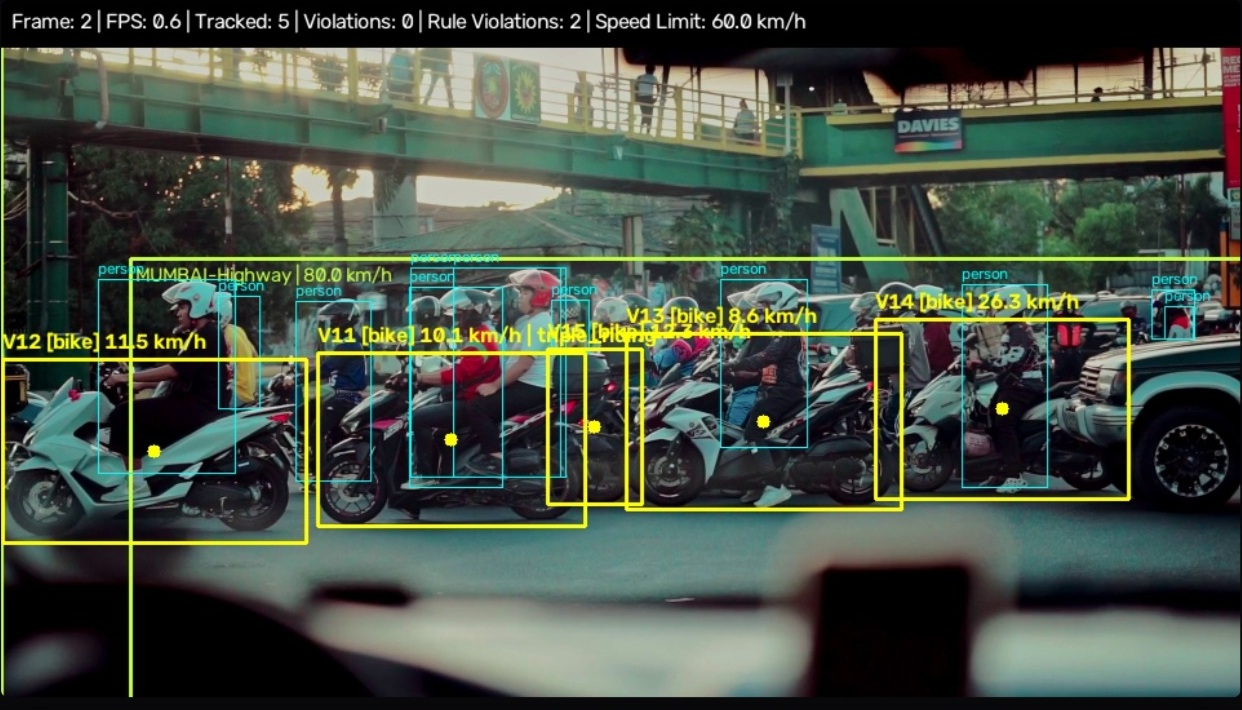
\includegraphics[width=0.9\columnwidth]{fig2a_dense_traffic.jpg}
\caption{Dense two-wheeler traffic: identities held under heavy mutual occlusion, with concurrent triple-riding flags
and per-vehicle speed labels.}
\end{subfigure}\\[4pt]
\begin{subfigure}{\columnwidth}\centering
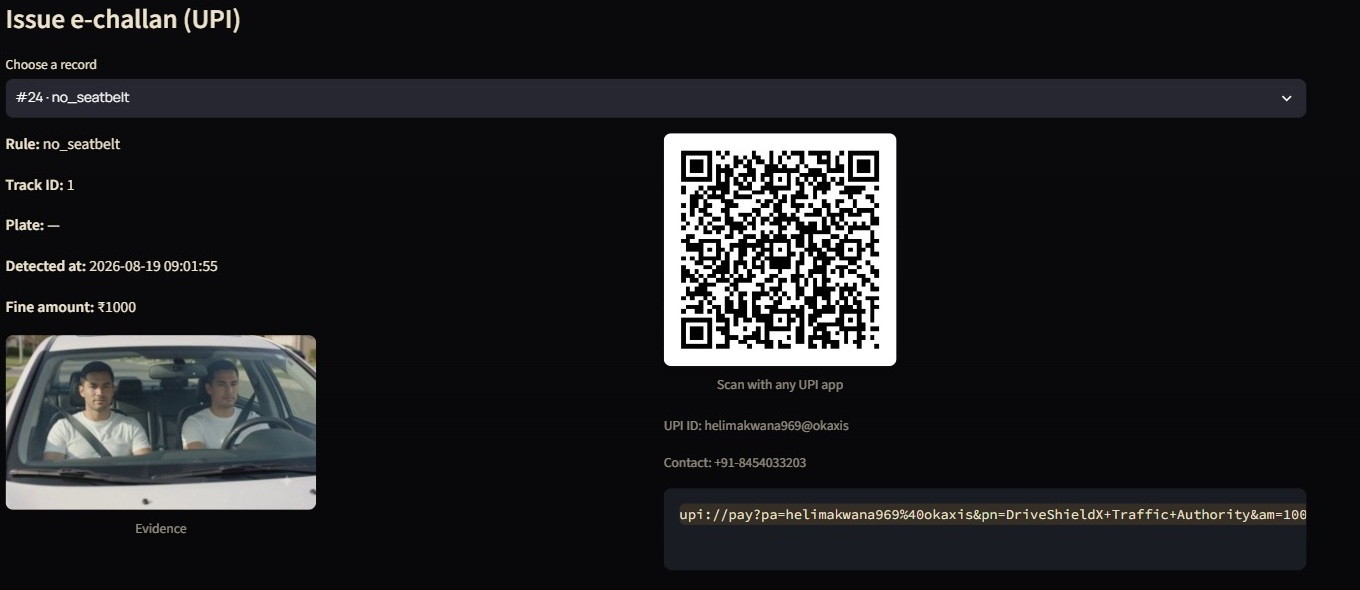
\includegraphics[width=0.9\columnwidth]{fig2b_seatbelt_evidence.jpg}
\caption{Seat-belt violation with its retained evidence crop. The plate field is empty; such an event is now not
issued automatically but routed to an officer.}
\end{subfigure}
\caption{Operation on real footage. Panel (a) is the hardest case in the set.}
\end{figure}

\begin{figure}[t]
\centering
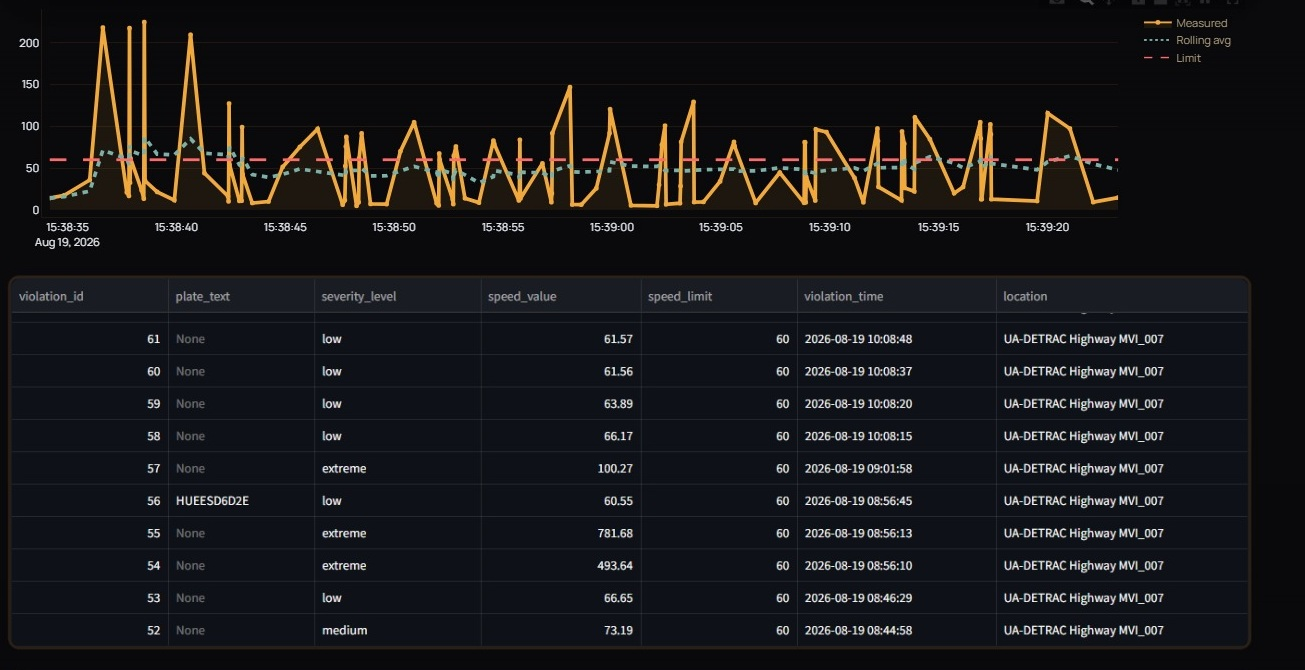
\includegraphics[width=0.9\columnwidth]{fig3_speed_failure.jpg}
\caption{Failure case, retained deliberately rather than omitted: speed telemetry against the 60 km/h limit, in which
the excursions above 200 km/h are artefacts of tracking and calibration rather than vehicles. Such
readings are now held for review instead of fined.}
\end{figure}

% ================================================================== 7
\section{Discussion}
\subsection{What the System Does Well}
The contribution that survives scrutiny is now both architectural and measured. Four violation types are evaluated
inside one inference cycle against one persistent vehicle identity, and ByteTrack keeps that identity with IDF1 75.2 on
public ground truth --- on a par with DeepSORT at a fraction of the cost. The disagreement gate gives the pipeline a
state published enforcement systems generally lack, and human review shows it removes almost all wrong automatic
challans. Registry verification closes the most damaging failure of automated e-challans, the notice sent to the wrong
citizen. Plate localisation (99.3\% on held-out photos), seat-belt detection (mAP@50 0.984) and the fog index (AUC 0.95)
are strong in their own right.

\subsection{Failure Cases}
\begin{itemize}
\item \textbf{Reading, not finding, limits attribution.} Plates are found in 99.3\% of photos but read exactly in
36.8\%. Unverified reads are routed to an officer, so the cost is officer time rather than wrong challans.
\item \textbf{Crashes on low-resolution CCTV.} The learned model finds 7 of 23 held-out crashes; most are still missed,
and the alert therefore goes to a person, not straight to an ambulance.
\item \textbf{Loose localisation propagates} into every crop-consuming stage; the helmet detector retains only 44\% of
its mAP@50 at mAP@50:95.
\item \textbf{Speed is consistent but not calibrated.} Tracking adds about 3 km/h of error; the scale constant and the
fixed frame rate dominate absolute error until per-camera calibration is done.
\item \textbf{Throughput.} 0.26--1.66 FPS on a CPU is far from multi-camera real time.
\end{itemize}

\subsection{Comparison with Existing Approaches}
We offer no numerical comparison against the systems surveyed in the literature review: those studies report on their own datasets
under their own capture conditions, and a table juxtaposing our 0.852 with a published 0.993 would imply a comparison
never performed. Against the e-challan systems already operating in India, the distinction DriveShieldX draws is in
capability: one record per vehicle across violations, a deferral state instead of automatic issuance on a disputed
prediction, no challan without a verified plate, repeat-offender and escalation logic that run themselves, and crash and
fog monitoring on the same cameras.

% ================================================================== 8
\section{Limitations and Outstanding Work}
\begin{itemize}
\item \textbf{Training corpora are not in hand.} Until they are recovered, no per-class precision, recall or F1 can be
reported for the detectors, and no dataset size or class balance can be stated.
\item \textbf{One training run per detector.} Mean $\pm$ standard deviation requires a seed sweep.
\item \textbf{Violation-level accuracy on video} for helmet, triple-riding and seat belt, and the ablations that depend
on it (aggregation, temporal confirmation, CLAHE), still need labelled video.
\item \textbf{Speed} needs per-zone calibration, the true frame rate read from the stream, and a field check against GPS
or radar.
\item \textbf{Plate reading} would benefit from fine-tuning the recogniser on Indian plates and from HD plate cameras.
\item \textbf{Crash detection} needs more and more varied training crashes than the 127 labelled here.
\item \textbf{Deployment prerequisites.} Official Vahan/Sarathi/Parivahan access (through NIC), DLT-registered SMS and
a government payment gateway; the demonstration uses test-mode Razorpay and an Android SMS gateway. Continuous
processing of public video carries data-protection obligations under the DPDP Act 2023: retention limits, access
control and an appeal route, which the contest window and officer review partly provide.
\end{itemize}

% ================================================================== 9
\section{Conclusion and Future Work}
DriveShieldX monitors road-safety violations with a single detection and tracking pipeline, binds every flag to one
persistent vehicle identity, and carries the record through plate reading and registry verification to an automated
challan, declining to issue when two models disagree or the plate cannot be verified. Measured on independent ground
truth, ByteTrack holds identities at IDF1 75.2, the gate cuts wrong automatic challans from 21.0\% to 1.1\%, plate
localisation reaches 99.3\% and exact reading 36.8\%, a learned crash model finds seven times as many held-out crashes
as the trajectory rules it replaces, and the fog index separates fog from clear footage with AUC 0.95. Its boundaries
are equally clear: plate reading and crash recall are the weakest stages, CPU throughput is 0.26--1.66 FPS, and the
speed scale is uncalibrated.

Future work follows from those boundaries: recover the corpora and re-validate per class; fine-tune plate reading on
Indian plates; calibrate speed per camera against a field reference; enlarge the crash training set; and measure
violation-level accuracy on labelled video. Only then do red-light and wrong-way violations, cross-camera identity
fusion and quantised edge deployment become worth pursuing.



\begin{figure*}[b]
\centering
\IfFileExists{pr_curves.pdf}{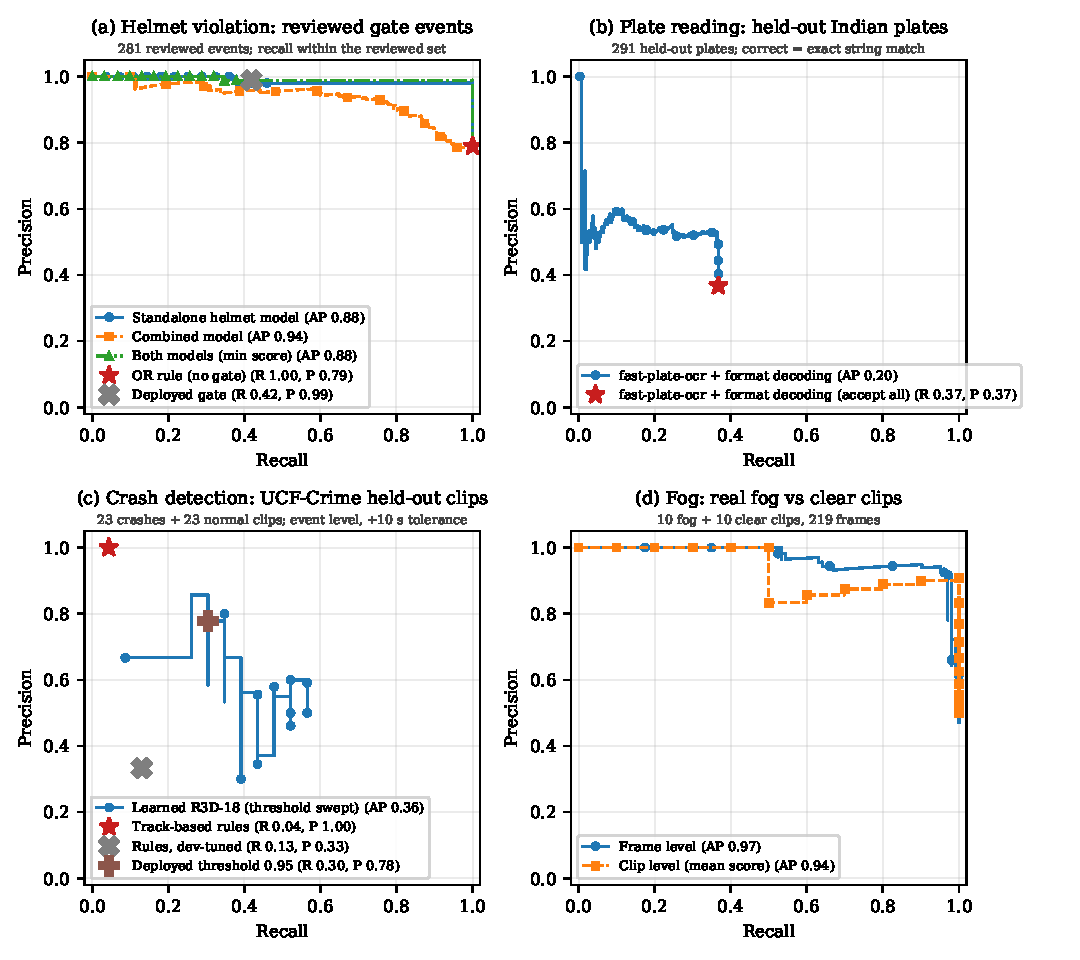
\includegraphics[width=0.78\textwidth,height=0.69\textwidth,keepaspectratio]{pr_curves.pdf}}{\fbox{\parbox[c][0.69\textwidth][c]{0.78\textwidth}{\centering\nm{Figure~4 is generated by \code{python -m evaluation.pr\_curves} from the project's labelled evaluations.}}}}
\caption{Precision versus recall on the project's labelled evaluations. (a) Helmet violation on the 281 human-reviewed
gate events, scored by the standalone model, the combined model and both together; the OR rule and the deployed gate are
marked. (b) Plate reading on 291 held-out Indian plates as the confidence needed to accept a read is raised. (c) Crash
detection on the UCF-Crime held-out clips at event level as the alarm threshold is swept, with the rule-based detectors
marked. (d) Fog versus clear at frame and clip level. AP = average precision.}
\end{figure*}

\section*{Acknowledgment}
The authors thank the Department of Computer Science and Technology, Usha Mittal Institute of Technology, SNDT Women's
University, for the guidance and resources provided during this work. DriveShieldX continues an earlier system,
OverSpeedX, from which the UA-DETRAC material is retained.

\section*{References}
{\scriptsize
\begin{enumerate}[leftmargin=1.6em,label={\arabic*.},itemsep=0pt]
\item Ultralytics, ``YOLOv8 documentation,'' 2023. https://docs.ultralytics.com
\item K.\,D.\ Dharmasaputra, B.\,P.\ Hartato, et al., ``Evaluation of YOLOv8 and centroid tracking in vehicle detection, classification, and counting system,'' Int.\ J.\ Intell.\ Syst.\ Appl., Oct.\ 2025.
\item S.\ Joshi, P.\ Jejure, C.\ Jadhav, and V.\ Jankar, ``Automatic number plate recognition using YOLOv8 model,'' Int.\ J.\ Sci.\ Res.\ Sci.\ Technol., 2025.
\item R.\ Srinath, J.\ Vrindavanam, S.\,Y.\,R., Y.\,L., and S.\,S.\ Chegaraddi, ``Smart vehicle recognition and e-challan generation system,'' Proc.\ INCET, 2020.
\item N.\ Wojke, A.\ Bewley, and D.\ Paulus, ``Simple online and realtime tracking with a deep association metric,'' Proc.\ IEEE ICIP, 2017, pp.\ 3645--3649.
\item Y.\ Zhang, P.\ Sun, Y.\ Jiang, D.\ Yu, Z.\ Yuan, P.\ Luo, and X.\ Wang, ``ByteTrack: Multi-object tracking by associating every detection box,'' Proc.\ ECCV, LNCS vol.\ 13682, Springer, 2022, pp.\ 1--21.
\item A.\ Bewley, Z.\ Ge, L.\ Ott, F.\ Ramos, and B.\ Upcroft, ``Simple online and realtime tracking,'' Proc.\ IEEE ICIP, 2016, pp.\ 3464--3468.
\item K.\ Bernardin and R.\ Stiefelhagen, ``Evaluating multiple object tracking performance: The CLEAR MOT metrics,'' EURASIP J.\ Image Video Process., vol.\ 2008, pp.\ 1--10, 2008.
\item E.\ Ristani, F.\ Solera, R.\ Zou, R.\ Cucchiara, and C.\ Tomasi, ``Performance measures and a data set for multi-target, multi-camera tracking,'' Proc.\ ECCVW, 2016, pp.\ 17--35.
\item J.\ Luiten, A.\ O\v{s}ep, P.\ Dendorfer, P.\ Torr, A.\ Geiger, L.\ Leal-Taix\'e, and B.\ Leibe, ``HOTA: A higher order metric for evaluating multi-object tracking,'' Int.\ J.\ Comput.\ Vis., vol.\ 129, no.\ 2, pp.\ 548--578, 2021.
\item A.\ Milan, L.\ Leal-Taix\'e, I.\ Reid, S.\ Roth, and K.\ Schindler, ``MOT16: A benchmark for multi-object tracking,'' arXiv:1603.00831, 2016.
\item C.-J.\ Lin and J.-Y.\ Jhang, ``Intelligent traffic-monitoring system based on YOLO and convolutional fuzzy neural networks,'' IEEE Access, vol.\ 10, pp.\ 14120--14133, 2022.
\item A.\,G.\ Suman, A.\,G., G.\ Raviteja, and G.\,R., ``An efficient deep learning model for helmet detection in real-world scenarios,'' Proc.\ ICSFT, 2026.
\item S.\ Sutikno, A.\ Sugiharto, and R.\ Kusumaningrum, ``Automated detection of driver and passenger without seat belt using YOLOv8,'' Int.\ J.\ Adv.\ Comput.\ Sci.\ Appl., 2023.
\item P.\,K.\ Gautam and S.\ Kumar, ``A centroid-based algorithm for measuring and tracking vehicle speed from a monocular camera using the YOLOv8 object detector,'' Indones.\ J.\ Electr.\ Eng.\ Comput.\ Sci., 2025.
\item R.\ Kejriwal, H.\,J.\ Ritika, A.\ Arora, and Mohana, ``Vehicle detection and counting using deep learning based YOLO and deep SORT algorithm for urban traffic management system,'' Proc.\ IEEE CONECCT, 2022, pp.\ 1--6.
\item M.\,R., M.\,R., R.\ Kiruthika, and G.\,S., ``Multi-task learning architecture for vehicle detection and tracking towards passenger safety and traffic violation detection,'' Proc.\ ICMLAS, 2025.
\item T.\ Qamar, N.\ Bawany, J.\ Shamsi, and K.\ Zahoor, ``Vision-based accident identification in traffic videos using deep learning,'' Suranaree J.\ Sci.\ Technol., 2024.
\item K.\ Zuiderveld, ``Contrast limited adaptive histogram equalization,'' in Graphics Gems IV, Academic Press, 1994, pp.\ 474--485.
\item JaidedAI, ``EasyOCR,'' 2023. https://github.com/JaidedAI/EasyOCR
\item L.\ Wen, D.\ Du, Z.\ Cai, Z.\ Lei, M.-C.\ Chang, H.\ Qi, J.\ Lim, M.-H.\ Yang, and S.\ Lyu, ``UA-DETRAC: A new benchmark and protocol for multi-object detection and tracking,'' Comput.\ Vis.\ Image Underst., vol.\ 193, 2020.
\item F.\ Wilcoxon, ``Individual comparisons by ranking methods,'' Biom.\ Bull., vol.\ 1, no.\ 6, pp.\ 80--83, 1945.
\item W.\ Sultani, C.\ Chen, and M.\ Shah, ``Real-world anomaly detection in surveillance videos,'' Proc.\ IEEE CVPR, 2018, pp.\ 6479--6488.
\item ankandrew, ``fast-plate-ocr: Fast and lightweight OCR for vehicle license plates,'' v1.1, MIT licence, 2026. https://github.com/ankandrew/fast-plate-ocr
\item ``Number Plate Identification Dataset,'' Bapatla Engineering College, Zenodo, 2024, doi:10.5281/zenodo.13954136 (CC-BY-4.0).
\item Government of India, ``The Motor Vehicles (Amendment) Act, 2019,'' Act No.\ 32 of 2019.
\item D.\ Tran, H.\ Wang, L.\ Torresani, J.\ Ray, Y.\ LeCun, and M.\ Paluri, ``A closer look at spatiotemporal convolutions for action recognition,'' Proc.\ IEEE CVPR, 2018, pp.\ 6450--6459.
\item W.\ Kay et al., ``The Kinetics human action video dataset,'' arXiv:1705.06950, 2017.
\item K.\ He, J.\ Sun, and X.\ Tang, ``Single image haze removal using dark channel prior,'' IEEE Trans.\ Pattern Anal.\ Mach.\ Intell., vol.\ 33, no.\ 12, pp.\ 2341--2353, 2011.
\end{enumerate}}
\end{document}
